%%%%%%%%%%%%%%%%%%%%%%% file template.tex %%%%%%%%%%%%%%%%%%%%%%%%%
%
% This is a template file for Web of Conferences Journal
%
% Copy it to a new file with a new name and use it as the basis
% for your article
%
%%%%%%%%%%%%%%%%%%%%%%%%%% EDP Science %%%%%%%%%%%%%%%%%%%%%%%%%%%%
%
%%%\documentclass[option]{webofc}
%%% "twocolumn" for typesetting an article in two columns format (default one column)
%
\documentclass{webofc}
%\documentclass[12pt]{article}
\usepackage[varg]{txfonts}   % Web of Conferences font
%\usepackage{bera}% optional: just to have a nice mono-spaced font
\usepackage{courier}
\usepackage{listings}  % for JSON in appendix
\usepackage{xcolor}
\usepackage{hyperref}
\usepackage[T1]{fontenc}
\usepackage[utf8]{inputenc}
\usepackage[english]{babel}

\usepackage{color}

\definecolor{darkred}{rgb}{0.5,0,0}
\definecolor{darkgreen}{rgb}{0,0.4,0}

\def\addt#1{\textcolor{darkgreen}{#1}}
\def\rmt#1{\textcolor{darkred}{#1}}

% forbid hyphen of words starting with capital letter
% http://tostudents.ru/2010/01/14/perenosy-slov-v-latex
\uchyph=0

\lstset{basicstyle=\footnotesize\ttfamily}
\definecolor{eclipseStrings}{RGB}{42,0.0,255}
\definecolor{eclipseKeywords}{RGB}{127,0,85}
\colorlet{numb}{magenta!60!black}

\lstdefinelanguage{json}{
    basicstyle=\footnotesize\ttfamily,
    commentstyle=\color{eclipseStrings}, % style of comment
    stringstyle=\color{eclipseKeywords}, % style of strings
    numbers=left,
    numberstyle=\scriptsize,
    stepnumber=1,
    numbersep=8pt,
    showstringspaces=false,
    breaklines=true,
%    frame=lines,
    backgroundcolor=\color{white}, %only if you like
}
%
% Put here some packages required or/and some personnal commands
%
%
\begin{document}
%
\title{Geant-val:

a web application for validation of detector simulations}
%
% subtitle is optionnal
%
%%%\subtitle{Do you have a subtitle?\\ If so, write it here}

\author{\firstname{Luc}~\lastname{Freyermuth}\inst{1} \and
        \firstname{Dmitri}~\lastname{Konstantinov}\inst{2,3}\fnsep\thanks{\email{Dmitri.Konstantinov@cern.ch}} \and
        \firstname{Grigorii}~\lastname{Latyshev}\inst{2}\fnsep\thanks{\email{Grigorii.Latyshev@cern.ch}} \and
        \firstname{Ivan}~\lastname{Razumov}\inst{2,3} \and %\fnsep\thanks{\email{Ivan.Razumov@cern.ch}}
        \firstname{Witold}~\lastname{Pokorski}\inst{3} \and %\fnsep\thanks{\email{Witold.Pokorski@cern.ch}}
        \firstname{Alberto}~\lastname{Ribon}\inst{3}%\fnsep\thanks{\email{Alberto.Ribon@cern.ch}}	
        % etc.
}
%\author{L.~Freyermuth \and D.~Konstantinov \and G.~Latyshev \and W.~Pokorski \and A.~Ribon}

\institute{L'École internationale des sciences du traitement de l'information, Cergy, France
\and
Institute for High Energy Physics named by A. A. Logunov of National Research Centre "Kurchatov Institute", Protvino, Russian Federation
\and
CERN
          }

\abstract{%
One of the key factors for the successful development of Monte-Carlo programs for physics simulations is to properly organize regression testing and validation. Geant4, the world-standard toolkit for HEP detector simulation, heavily relies on this activity. The CERN SFT group, which contributes to the development, testing, deployment and support of the toolkit, is also in charge of running on a monthly basis a set of community-developed tests using the development releases of Geant4.
We present the web application \textsf{Geant-val} developed for visualizing the results of these tests so that comparisons between different Geant4 releases can be made. The application is written using Express.js, Node.js and Angular frameworks, and uses PostgreSQL for storing test results. Test results are visualised using ROOT and JSROOT. In addition to pure visual comparisons, we perform different statistical tests ($\chi^2$, Kolmogorov-Smirnov, etc) on the client side using JavaScript Web Workers.
}
%
\maketitle
%
\section{Introduction}
\label{sec-introduction}
Geant4~\cite{Geant4} is a toolkit for the simulation of the passage of particles through matter. Its areas of application include high energy, nuclear and accelerator physics, as well as studies in medical and space science.

The Geant4 team produces a public release once a year, with monthly internal development releases. These releases need to be validated.

Physics validation of Geant4 includes regression testing (comparing physics output from one release to another), comparison of performance between different physics models and validation testing (comparing physics output with published experimental results). As a result it requires analysing
% TODO: data -> cases? output files?
a large amount of data produced by Geant4 tests.

%These tests were developed by Geant4 community, and utilise various approaches and a wide stack of technologies, such as PHP, C++, Python and others. This diversity makes it very hard to quickly perform full validation of release, as it requires running all developer's micro frameworks and merging data into one view. In addition, different formats of experimental data are often used, and that prevents sharing the same data between tests.

% In this article we present a tool to perform statistical and visual validation of different Geant4 physics models and releases. % comparisons with respect to previous release(s) and to the experimental data.

%The presented tool is a website working with a special framework designed for Geant4 tests configuration and execution.

% Geant4 validation procedure consists of two steps: generating results (executing the tests and importing their output into Geant-val) and analysing these results.

\section{Requirements}
\label{sec:requirements}

requirements

\section{Components of validation system}
\label{sec-webapplication}

The components of \textsf{Geant-val} web application and interactions between them are shown in the Fig.~\ref{fig:dataflow}.

\begin{figure}[h]
    \centering
    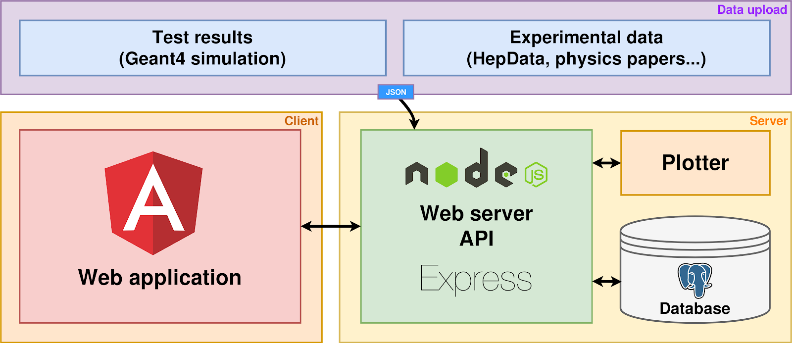
\includegraphics[width=0.8\textwidth,clip]{schema.png}
    \caption{Components of \textsf{Geant-val} web application and flow of data between them.}
    \label{fig:dataflow}
\end{figure}

\textbf{The server} is the core of the Geant4 validation system. It provides a web API that allows clients to access the database, respond to the clients' requests and generate high quality plots "on the fly" whenever they are requested using the ROOT~\cite{ROOT} data analysis framework.
It is written in JavaScript and runs with the Node.js engine~\cite{NodeJS}. 

\textbf{The database} is used for storing plots containing simulation results or experimental data, together with parameters describing these plots: tool name and version (e.g. \texttt{Geant4, 10.4.p02}), name of the test by which the plot was produced, or Inspire (HepData) ID of the article, etc. PostgreSQL~\cite{Postgre} is used as database management system for the application. The database instance is provided by the CERN Database-On-Demand service  % The database schema is designed in a way to allow scatter plots and histograms with unlimited number of optional test parameters in additional to a few mandatory ones to be stored.

% db schema

\textbf{A ROOT-based C++ plotting utility} was developed to produce high quality plots. It uses data in the JSON format which has been introduced as main interchange format between all parts of the application. The utility is not deeply integrated in the server infrastructure and can be used as a standalone application. It supports all types of application's data, can plot histograms with different binning on one canvas, and produce ratio plots. Ranges and scales of plot axes are selected automatically, with ability to override if necessary. % User-defined styles are also supported.

\textbf{Web interface} is user-friendly AngularJS~\cite{AngularJS} single page application which provides plots with tests results together with statistical analysis to the users.

%AngularJS is chosen because it allows to build efficient web applications with highly reusable components.

% The SPA contains 2 pages (see~\ref{sec-analyse} for details):
% \begin{itemize}
%     \item User layouts
%     \item Statistical comparisons
% \end{itemize}

%\begin{figure}[h]
%    \centering
%    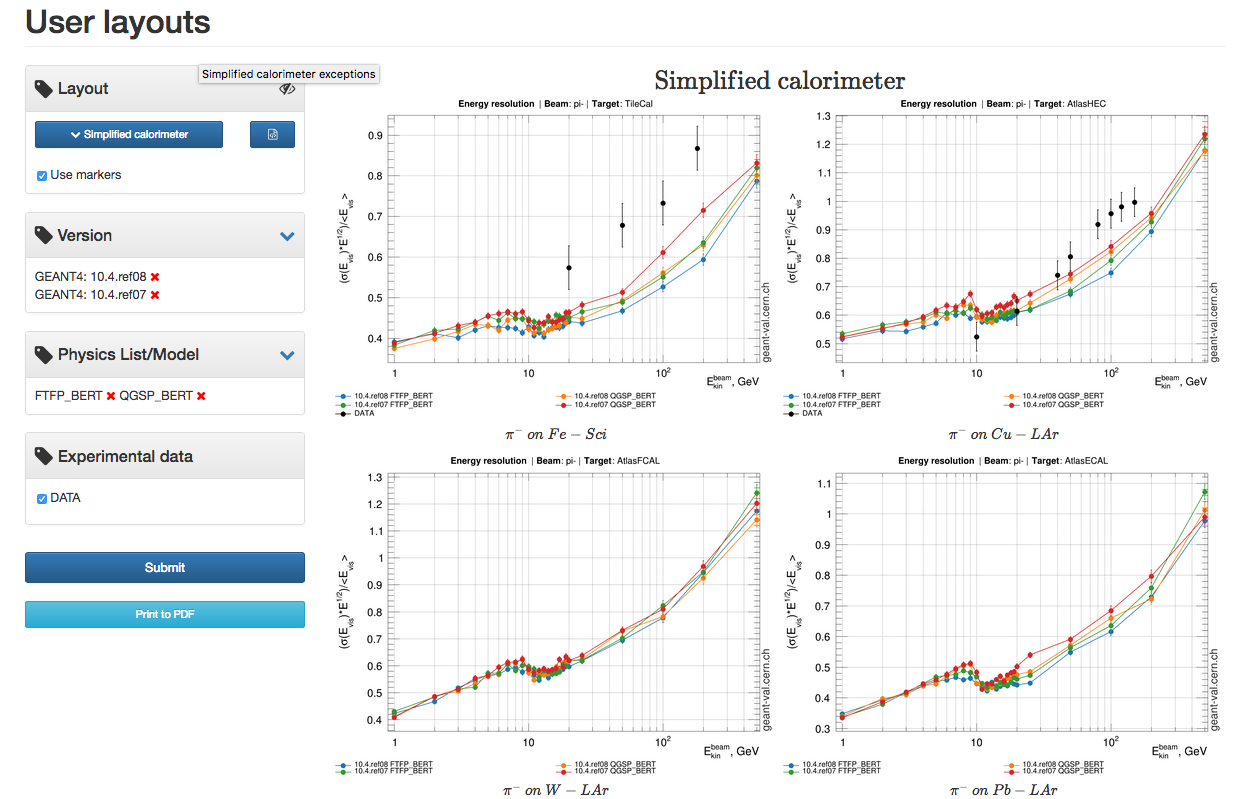
\includegraphics[width=0.8\textwidth,clip]{layout_sc.png}
%    \caption{Example of user defined layout for the Geant4 "simplified calorimeter" test showing test results for two Geant4 reference releases - 10.4.ref07 and 10.4.ref08.}
%    \label{fig:layouts}
%\end{figure}

%\textit{User layouts} page (see Fig.~\ref{fig:layouts}). Some Geant4 tests produce hundreds of different plots, but for fast "visual" validation it is often enough to compare only a small well-defined subset of them. The \textit{User layout} is an XML file describing what plots should be displayed and how should they be laid out on a page. User can use one of the existing layouts or define their own one (see Appendix~\ref{adx:XML-format}).
% is used to perform fast visual validation of Geant4.  
% One can use one of the existing templates or create and upload their own one. 
% It is possible to compare different versions between themselves or against experimental data. 
% If two or more Geant4 versions are selected, one can also select a "reference" dataset and plot the ratio of other datasets to it.

%\begin{figure}[h]
%    \centering
%    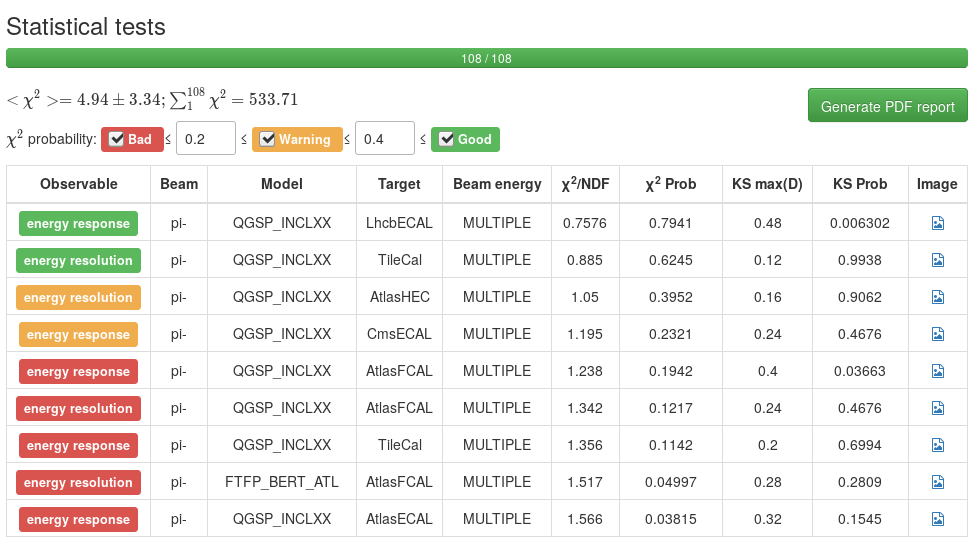
\includegraphics[width=0.8\textwidth,clip]{statcomparison.png}
%    \caption{Example of statistical comparison between two official Geant4 releases, 10.5.beta01 and 10.4.p02, for the "simplified calorimeter" test.}
%    \label{fig:statcomparison}
%\end{figure}

%\textit{Statistical comparisons} page (see Fig.~\ref{fig:statcomparison}) allows one to perform comparison of simulation with compatible experimental results using statistical tests. It displays results of statistical comparison for pairs of plots with the same parameters' values.
%Currently $\chi^2$ ($\chi^2/n.d.f.$, $\chi^2$ probability) and Kolmogorov-Smirnov (KS Max(D), KS probability) tests are implemented. All computations are performed asynchronously on the client side using JavaScript WebWorkers.
%For this purpose, JavaScript code to perform $\chi^2$ and Kolmogorov-Smirnov tests have been written, and their results cross-checked against the same statistical techniques implemented in the ROOT framework.


%On the \textit{experimental data} page (see Fig.~\ref{fig:exppage}) a summary table of available experimental data is displayed. The data is extracted from original articles or imported from HepDATA~\cite{hepdata} portal. % The experimental data is not linked with particular test and can be used by any tests if parameters match with simulation data.

%\begin{figure}[h]
%    \centering
%    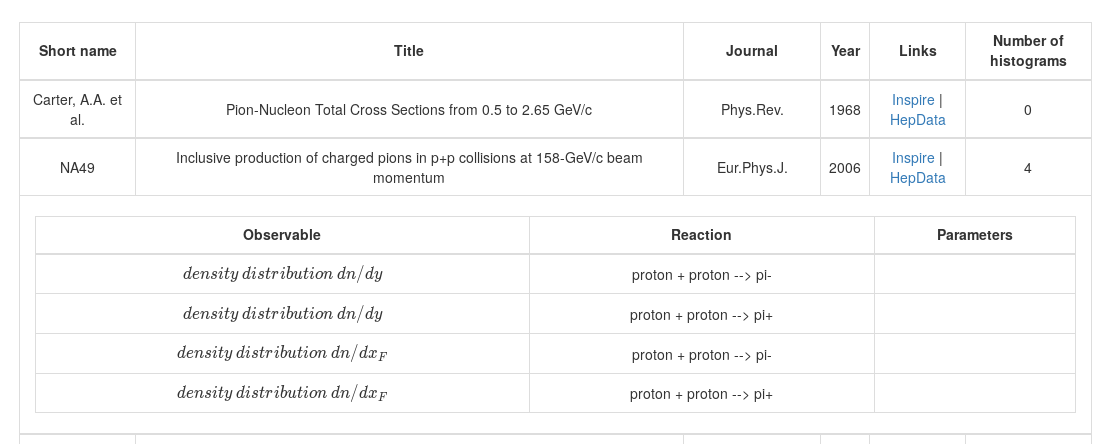
\includegraphics[width=0.8\textwidth,clip]{expdata.png}
%    \caption{Available experimental data.}
%    \label{fig:exppage}
%\end{figure}

Each plot on the website can be displayed as a static image produced by {\tt plotter} or as an interactive JSROOT~\cite{JSROOT} object, which allows changing axes ranges, scales and styles of the data "on the fly" in the same way as it can be done in ROOT. It is possible to export the plots in PNG, ROOT, EPS, Gnuplot~\cite{gnuplot} or \textsf{Geant-val} JSON format. 

Access to the test results produced with internal Geant4 releases is restricted to the Geant4 developers authenticated via CERN Single Sign-On. For public Geant4 releases the access is open to anyone.

%Don't forget to give each section, subsection, subsubsection, and
%paragraph a unique label (see Sect.~\ref{sec-1}).

%For one-column wide figures use syntax of figure~\ref{fig-1}
%\begin{figure}[h]
% Use the relevant command for your figure-insertion program
% to insert the figure file.
%\centering
%\includegraphics[width=1cm,clip]{tiger}
%\caption{Please write your figure caption here}
%\label{fig-1}       % Give a unique label
%\end{figure}

%For two-column wide figures use syntax of figure~\ref{fig-2}
%\begin{figure*}
%\centering
% Use the relevant command for your figure-insertion program
% to insert the figure file. See example above.
% If not, use
%\vspace*{5cm}       % Give the correct figure height in cm
%\caption{Please write your figure caption here}
%\label{fig-2}       % Give a unique label
%\end{figure*}

%For figure with sidecaption legend use syntax of figure
%\begin{figure}
% Use the relevant command for your figure-insertion program
% to insert the figure file.
%\centering
%\sidecaption
%\includegraphics[width=5cm,clip]{tiger}
%\caption{Please write your figure caption here}
%\label{fig-3}       % Give a unique label
%\end{figure}

%For tables use syntax in table~\ref{tab-1}.
%\begin{table}
%\centering
%\caption{Please write your table caption here}
%\label{tab-1}       % Give a unique label
% For LaTeX tables you can use
%\begin{tabular}{lll}
%\hline
%first & second & third  \\\hline
%number & number & number \\
%number & number & number \\\hline
%\end{tabular}
% Or use
%\vspace*{5cm}  % with the correct table height
%\end{table}

To manage a set of Geant4 tests and their configurations, a \textbf{{\tt mc-config-generator} framework} was developed. It allows one to configure and run test jobs in various batch systems (CERN LSF, HTCondor, Torque PBS), and to convert the results into  JSON format for further uploading to the application database. The framework is not Geant4-specific, and can be used with other projects (e.g., Pythia8). Source code is available in corresponding Git repository\footnote{https://gitlab.cern.ch/GeantValidation/geant-config-generator}.



% \vfill\break
\section{Web application data model}

A \textit{plot} is a central element of the data model of \textsf{Geant-val} application. Each plot consists of:
\begin{itemize}
    \item Arrays describing one-dimensional histograms or scatter plots;
    \item Name of the measured physics value (\textit{observable}), which used for matching \textit{plot} to the experimental data (e.g., differential cross-section);
    \item The name and version of tool (e.g., Geant4 and 10.5.beta01);
    \item Name of the test (e.g. Tileatlas);
    \item Name(s) and value(s) of the parameters used for running the test (e.g. Physics List: FTFP\_BERT);
    \item For experimental data, Inspire~\cite{inspire} or HepDATA~\cite{hepdata} ID of the original article.
\end{itemize}

\section{User interface}
\label{sec-analyse}

The \textsf{Geant-val} website provides two ways of viewing and comparing results:

\begin{itemize}



\item \textit{Statistical comparisons} page allows one to perform comparison of simulation with compatible experimental results using statistical tests and visually. % It displays results of statistical comparison for pairs of plots with the same parameters' values.

In visual mode  (see Fig.~\ref{fig:sc_visual_ratio}) one can select various parameters in left side drop down menu and request plots corresponding selected values. In this mode page it is possible to mark one Geant4 release as "reference" to get ratio plots between several results.

In statistical mode (see Fig.~\ref{fig:statcomparison}) the page shows results of $\chi^2$ ($\chi^2/n.d.f.$, $\chi^2$ probability) and Kolmogorov-Smirnov (KS Max(D), KS probability) tests between two Geant4 releases for all matching pairs of test results.
All computations are fast and performed asynchronously on the client side using JavaScript WebWorkers. For this purpose, JavaScript code to perform $\chi^2$ and Kolmogorov-Smirnov tests have been written, and their results cross-checked against the same statistical techniques implemented in the ROOT framework ({\tt ROOT::TH1::Chi2Test()} and {\tt ROOT:TMath::KolmogorovTest()} correspondingly).

Users can specify range of $\chi^2$ probability to mark results with ''bad'', ''warning'' and ''good''. Further it is possible to download PDF report with plots with selected classification.

\begin{figure}[h]
    \centering
    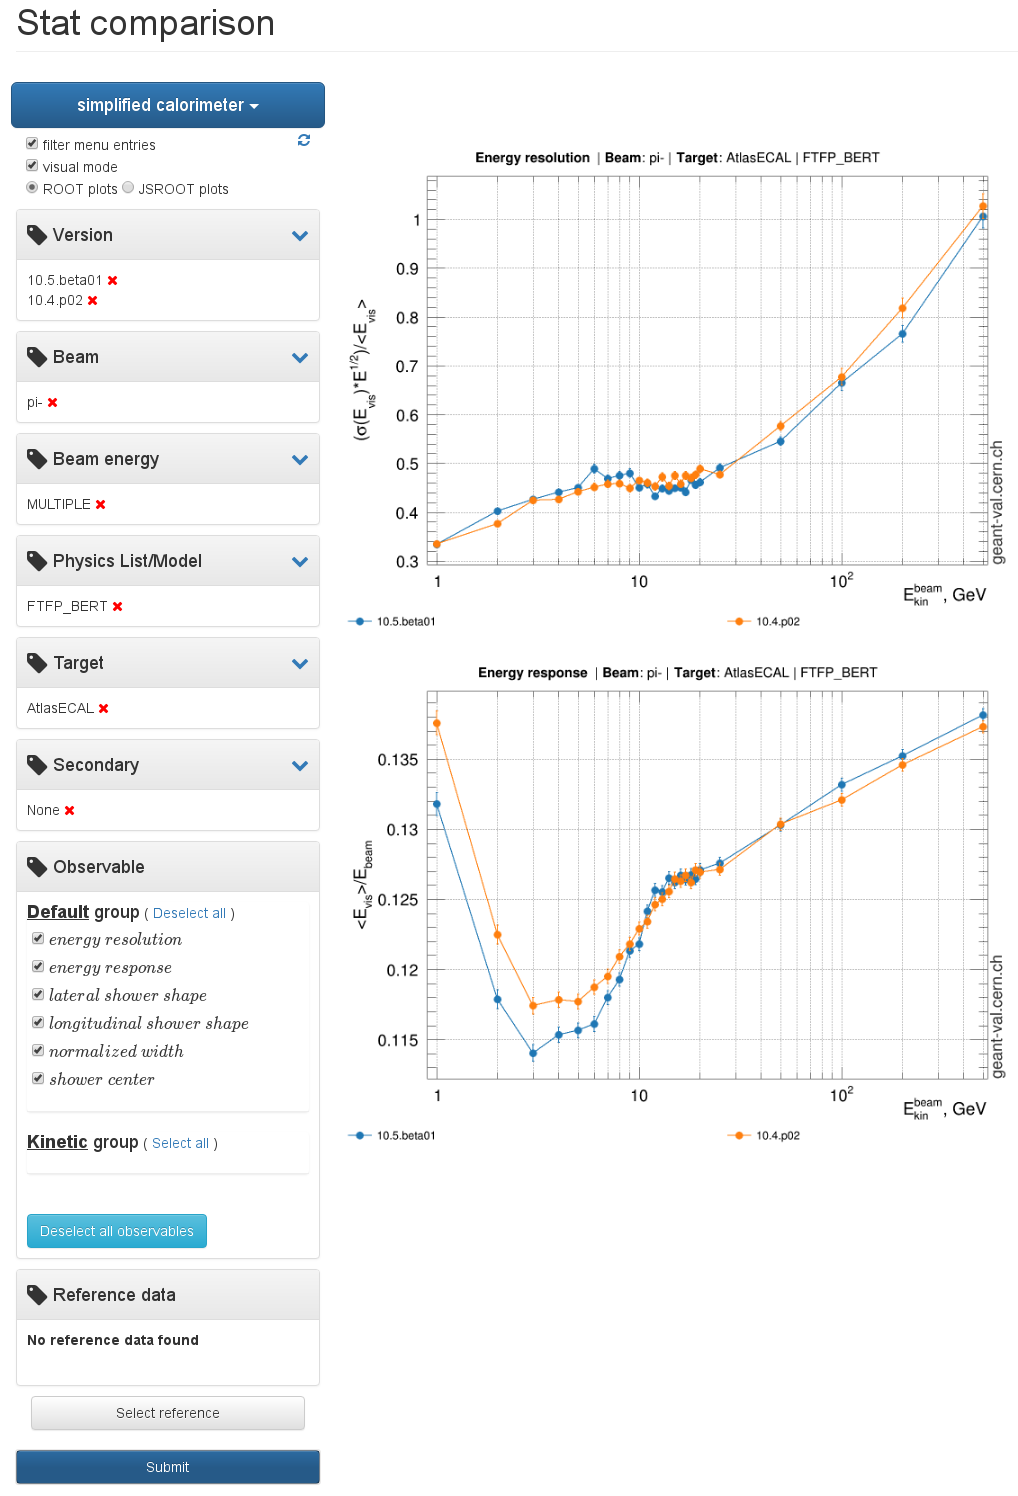
\includegraphics[width=0.8\textwidth,clip]{sc_visual_ratio.png}
    \caption{Plots of "simplified calorimeter" test results for Geant4 releases 10.5.beta01 and 10.4.p02 with 10.5.beta01 selected as "reference".}
    \label{fig:sc_visual_ratio}
\end{figure}

\begin{figure}[h]
    \centering
    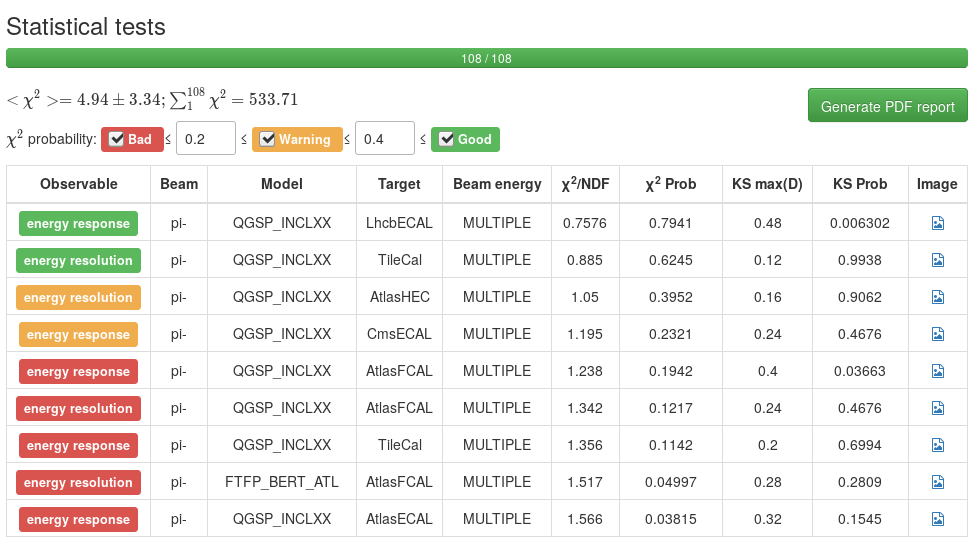
\includegraphics[width=0.8\textwidth,clip]{statcomparison.png}
    \caption{Statistical comparison of "simplified calorimeter" test results between Geant4 releases 10.5.beta01 and 10.4.p02 for $\pi-$ beam.}
    \label{fig:statcomparison}
\end{figure}



\item \textit{User layouts} page (see Fig.~\ref{fig:layouts}). Some Geant4 tests produce hundreds of different plots, but for fast "visual" validation it is often enough to compare only a small well-defined subset of them. On the page user needs just to select layout to be used, Geant4 version(s) and physics list(s) and experimental data to be used. All other plot's parameters should be defined in layout file. It allows to perform fast and clear visual comparing of several Geant4 versions/physics lists. For all plots there is possibility to request ratio plots to see difference between them in detail.

The \textit{layout} is an XML file describing what plots should be displayed and how should they be laid out on a page. We provide layouts for integrated tests however users can define and use on the website their own one.

\begin{figure}[h]
    \centering
    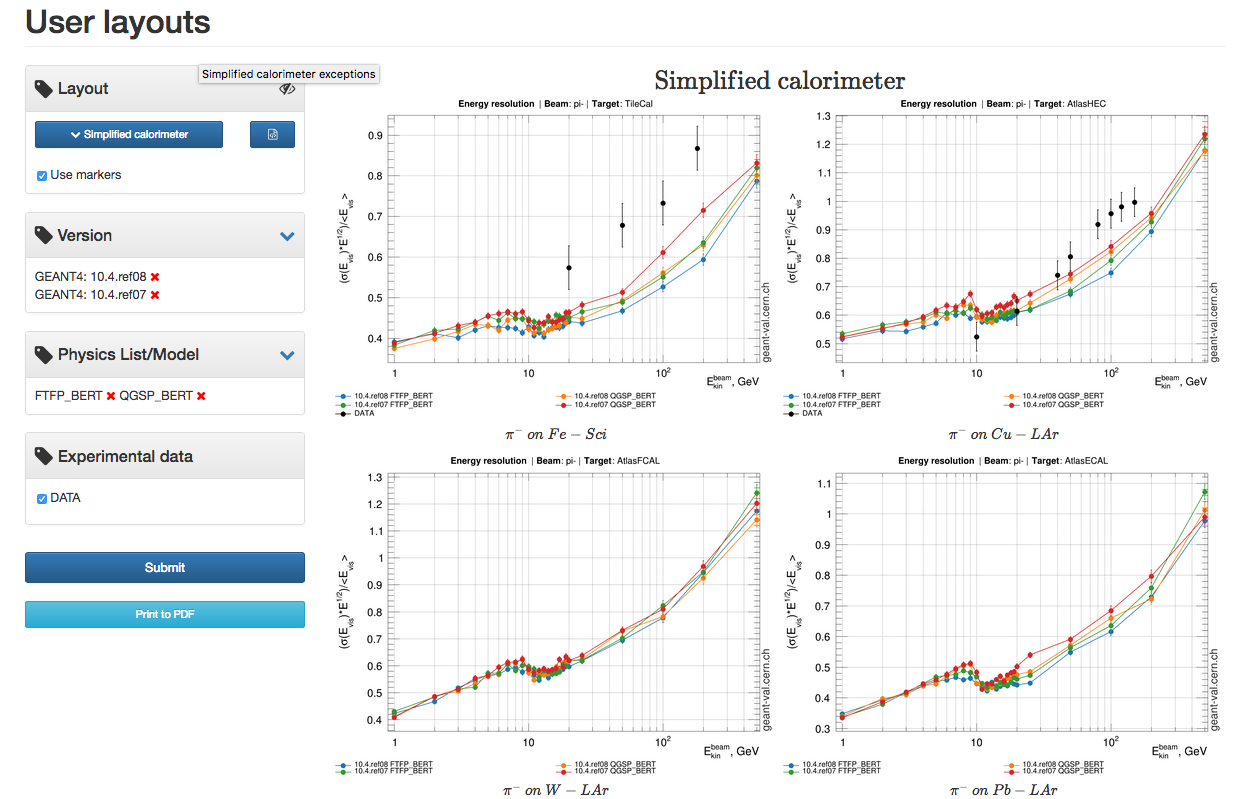
\includegraphics[width=0.8\textwidth,clip]{layout_sc.png}
    \caption{Layout for the Geant4 "simplified calorimeter" test with results for Geant4 reference releases 10.4.ref07, 10.4.ref08 and physics lists FTFP\_BERT and QGSP\_BERT.}
    \label{fig:layouts}
\end{figure}

\end{itemize}

In both comparison modes users can change plot's axes ranges/scales and download them in PNG, EPS, ROOT formats. Raw plot's data in Gnuplot and the website's JSON formats are also accessible.

% \section{Validation work flow}
\label{sec-workflow}

To perform Geant4 validation using given test one needs to run test, convert test's output to Geant validation JSON format (see Appendix~\ref{adx:JSON-format}) and upload produced files to the website.

To build a test it is possible to use CERN Gitlab repository\footnote{https://gitlab.cern.ch/GeantValidation/geant-validation-tests}, which provides a simple way to compile the test for any Geant4 version (if the test supports requested version of Geant4).
Then one needs to integrate the test in {\tt mc-config-generator} system to be able produce and parse tests results.

Uploading of JSON files is performed by {\tt geant\_upload.py}\footnote{https://gitlab.cern.ch/GeantValidation/GVP/raw/master/scripts/geant\_upload.py} console utility.
After uploading the results are available on the website to view and analyze.


% To manage a set of Geant4 tests and their configurations Python framework {\tt mc-config-generator} is developed. It allows to configure and run test jobs in batch system (CERN LSF, HTCondor, Torque PBS), and parse simulation results to JSON format for further uploading to the application database.
The framework is not Geant4-specific, and can be used with other projects (e.g., Pythia8). Source code is available on
CERN Gitlab repository\footnote{https://gitlab.cern.ch/GeantValidation/geant-config-generator}.

To be used in Geant validation application two test related parts should be added in {\tt mc-config-generator} system:

\begin{itemize}
	\item Parameters description file and templates for test run;
	\item Python class for converting test output to the application's JSON format (see Appendix~\ref{adx:JSON-format}).
\end{itemize}

According to test's parameters and template files {\tt mc-config-generator} generates Cartesian product of input parameters and store prepared configurations in "jobs". Later the jobs can be submitted in batch system or run locally. In additional {\tt mc-config-generator} provides console commands to monitor status of jobs and measure execution time for each job.

The Python parser class should be written for test to convert test's results to the application JSON files. Further these JSON files can be uploaded to the website to be available for Geant4 validation.
Convert procedure is automatically paralleled over all available CPU to gain maximum execution speed.
% Python parse class inherits from $BaseParser$ class as listed in example below:

% \begin{lstlisting}[language=python,firstnumber=1]
% #!/usr/bin/env python
% from gts.BaseParser import BaseParser
% from gts.utils import getJSON

% class Test(BaseParser):
%     TEST = "TestName"
%     IGNOREKEYS = []

%     def parse(self, jobs):
%         # your code here
%         yield getJSON(...)
% \end{lstlisting}



%\subsection{Geant tests repository}
%\label{sec-geant-validation-tests}

%Sometimes we have to modify original tests developed by Geant4 community to either make their output more suitable for parsing or to fix some unsafe behaviour (like using default physics model). These modified tests are kept in CERN Gitlab repository\footnote{https://gitlab.cern.ch/GeantValidation/geant-validation-tests}.

%We have also developed tools to build all test for a given Geant4 release or releases.
%Also we wrote build system to have a possibility to build tests for all Geant4 releases (if test supports it). In additional {\tt geant-validation-tests} build system encapsulates debug information in each test (compile flags and git hash) to simplify test's debugging.

% \section{Current status}
\label{sec-status}

The web application and {\tt geant-config-generator} framework are ready to use by Geant4 test developers. The website is passed security audit by CERN IT department.

At the moment 12 Geant4 tests are fully integrated in Geant Validation system and have layouts on the website (see Table~\ref{table:tests}):

\begin{table}[h]
\centering
\begin{tabular}{lll}
\hline
Author & Tests  \\\hline
Vladimir Ivanchenko & FluctTest, MscHanson, TestEm3, TestEm9, Hadr00, \\ 
& Test22~(HARP, NA49, NA61), Test37, Test46, Tileatlas \\
Susanna Guatelli, David Bolst & FragTest \\
Andrea Dotti, Alberto Ribon & Simplified calorimeter \\
Alexander Howard & Test15 \\

\end{tabular}
\caption{Tests integrated in Geant Validation website.}
\label{table:tests}
\end{table}

%\begin{itemize}
%    \item FluctTest (Vladimir Ivanchenko)
%    \item FragTest (Susanna Guatelli, David Bolst)
%    \item MscHanson (Vladimir Ivanchenko)
%    \item TestEm3 (Vladimir Ivanchenko)
%    \item TestEm9 (Vladimir Ivanchenko)
%    \item Hadr00 (Vladimir Ivanchenko)
%    \item Simplified calorimeter (Andrea Dotti, Alberto Ribon)
%    \item Test15 (Alexander Howard)
%    \item Test22~(HARP, NA49, NA61) (Vladimir Ivanchenko)
%    \item Test37 (Vladimir Ivanchenko)
%    \item Test46 (Vladimir Ivanchenko)
%    \item Tileatlas (Vladimir Ivanchenko)
%\end{itemize}
%FluctTest, FragTest, MscHanson, TestEm3, TestEm9, Hadr00, simplified calorimeter, test15, test22~(HARP, NA49, NA61), test37, test46, tileatlas. 

Currently the application's database contains 86213 tests histograms and charts as well as 1414 experimental datasets.

The web application is distributed using Docker technology and can be easily deployed on any operating system.

There are major tasks to be done in the future:
\begin{itemize}
	\item Migrate client side of the application to Angular2+ framework;
	\item Add more Geant4 tests and tests from other projects;
	\item Improve statistical comparison page;
	\item Improve {\tt geant-config-generator} framework;
\end{itemize}

\section{Conclusion}
\label{sec-status}

The presented software provides an uniform and clear way of performing all stages of physics validation: from creating configuration files and running simulation code to producing final plots.

The \textsf{Geant-val} web application and the {\tt mc-config-generator} framework are actively used by Geant4 developers in CERN and by Geant4 Medical Simulation Benchmark Group (G4BSMG).


% At the moment, 12 Geant4 tests are fully integrated in Geant Validation system and have layouts on the website (see Table~\ref{table:tests}):

% \begin{table}[h]
% \centering
% \begin{tabular}{lll}
% \hline
% Author & Tests  \\\hline
% Vladimir Ivanchenko & FluctTest, MscHanson, TestEm3, TestEm9, Hadr00, \\ 
% & Test22~(HARP, NA49, NA61), Test37, Test46, Tileatlas \\
% Susanna Guatelli, David Bolst & FragTest \\
% Andrea Dotti, Alberto Ribon & Simplified calorimeter \\
% Alexander Howard & Test15 \\

% \end{tabular}
% \caption{Tests integrated in Geant Validation website.}
% \label{table:tests}
% \end{table}

% Currently, the application's database contains 86213 test histograms and charts as well as 1414 experimental datasets.

% \pagebreak
\begin{thebibliography}{}
%
% and use \bibitem to create references.
%
\bibitem{Geant4}
S.~Agostinelli {\it et al.} [GEANT4 Collaboration],
  %``GEANT4: A Simulation toolkit,''
  Nucl.\ Instrum.\ Meth.\ A {\bf 506}, 250 (2003).
  doi:10.1016/S0168-9002(03)01368-8
  %%CITATION = doi:10.1016/S0168-9002(03)01368-8;%%

\bibitem{inspire}
INSPIRE-HEP: High-Energy Physics Literature Database \url{http://inspirehep.net/}

\bibitem{hepdata}
  E.~Maguire, L.~Heinrich and G.~Watt,
  %``HEPData: a repository for high energy physics data,''
  J.\ Phys.\ Conf.\ Ser.\  {\bf 898} (2017) no.10,  102006
  doi:10.1088/1742-6596/898/10/102006
  [arXiv:1704.05473 [hep-ex]].
  %%CITATION = doi:10.1088/1742-6596/898/10/102006;%%
  %13 citations counted in INSPIRE as of 26 Oct 2018

\bibitem{ROOT}
    Rene Brun and Fons Rademakers,
    ROOT - An Object Oriented Data Analysis Framework,
    Proceedings AIHENP'96 Workshop, Lausanne, Sep. 1996, Nucl. Inst. \& Meth. in Phys. Res. A 389 (1997) 81-86. See also (\url{http://root.cern.ch}).

\bibitem{NodeJS}
NodeJS is a JavaScript runtime \url{https://nodejs.org/}

\bibitem{Postgre}
PostgreSQL is an open-source database \url{https://www.postgresql.org/}

\bibitem{AngularJS}
AngularJS is an MWM JavaScript framework \url{https://angularjs.org/}
%AngularJS, v.1.4.8, 20.11.2015, \url{https://github.com/angular/angular.js/commit/75e876424da5f569481488d03cf3a61441341513}

\bibitem{JSROOT}
Bertrand Bellenot and Sergey Linev 2015, J. Phys.: Conf. Ser.,664,  062033

\bibitem{gnuplot}
Gnuplot is a portable command-line driven graphing utility \url{http://www.gnuplot.info/}

\end{thebibliography}

% % reset numbering and title
\setcounter{figure}{0}
\renewcommand{\figurename}{Appendix}

\definecolor{eclipseStrings}{RGB}{42,0.0,255}
\definecolor{eclipseKeywords}{RGB}{127,0,85}
\colorlet{numb}{magenta!60!black}

\lstdefinelanguage{json}{
    basicstyle=\normalsize\ttfamily,
    commentstyle=\color{eclipseStrings}, % style of comment
    stringstyle=\color{eclipseKeywords}, % style of strings
    numbers=left,
    numberstyle=\scriptsize,
    stepnumber=1,
    numbersep=8pt,
    showstringspaces=false,
    breaklines=true,
%    frame=lines,
    backgroundcolor=\color{white}, %only if you like
}

\begin{figure}

\begin{lstlisting}[language=json,firstnumber=1]
{
  "article": {"inspireId": -1},
  "mctool": {"name": "Geant4", "version": "", "model": ""},
  "testName": "",
  "metadata": {"observableName": "", "reaction": "",
    "targetName": "", "beamParticle": "",
    "beamEnergies": [], "secondaryParticle": "",
    "parameters": [
      {
        "names": "THETA",
        "values": "60 degrees"
      }
    ]
  },
  // for scatter data
  "plotType": "SCATTER2D",
  "chart": {
    "nPoints: 0,
    "title": "", "xAxisName": "", "yAxisName": "",
    "xValues": [], "yValues": [],
    "xStatErrorsPlus": [], "xStatErrorsMinus": [],
    "yStatErrorsPlus": [], "yStatErrorsMinus": [],
    "xSysErrorsPlus": [], "xSysErrorsMinus": [],
    "ySysErrorsPlus": [], "ySysErrorsMinus": []
  },
  // for histogram data
  "plotType": "TH1",
  "histogram": {
    "nBins: [0],
    "title: "", "xAxisName": "", "yAxisName": "",
    "binEdgeLow": [], "binEdgeHigh": [], "binContent": [],
    "yStatErrorsPlus": [], "yStatErrorsMinus": [],
    "ySysErrorsPlus": [], "ySysErrorsMinus": [],
    "binLabel": []
  }
}
\end{lstlisting}

\caption{Example of JSON format used by the web application.}
\label{adx:JSON-format}
\end{figure}

%\begin{figure}
%\begin{lstlisting}
%/control/verbose 1
%/run/verbose 1
%/tracking/verbose 0
%/testhadr/TargetMat G4_%TARGETELM%
%/testhadr/TargetRadius 2 cm
%/testhadr/TargetLength  50 cm
%/run/printProgress 10
%/run/initialize
%/process/em/workerVerbose 0
%/run/setCut 1 km
%/gun/particle proton
%/gun/energy 20. GeV
%/testhadr/targetElm %TARGETELM%
%/testhadr/particle %PARTICLE%
%/testhadr/fileName test
%/testhadr/verbose 1
%/run/beamOn 1
%\end{lstlisting}
%\caption{Template file for "Hadr00" test.}
%\label{hadr00-template}
%\end{figure}

%\begin{figure}
%\begin{lstlisting}
%!PARTICLE=proton, e-, kaon-, kaon+, neutron, pi-, pi+, gamma
%!TARGETELM=Be, C, Cu, Fe, H, Pb, Si, U, He, Al
%!PHYSICS_LIST=FTFP_BERT, QGSP_BERT, FTFP_BERT_HP, FTFP_BERT_TRV, QGSP_BIC, QBBC
%PARTICLE | TARGETELM | PHYSICS_LIST
%PARTICLE | TARGETELM | PHYSICS_LIST
%\end{lstlisting}
%\caption{Parameter's file for "Hadr00" test.}
%\label{hadr00-parameters}
%\end{figure}


%\begin{figure}
%
%\begin{verbatim}
%#!/bin/bash
%source config.sh
%export PHYSLIST="%PHYSICS_LIST%"
%Hadr00 Hadr00.mac 1>test_stdout.txt 2>test_stderr.txt
%\end{verbatim}
%\caption{Run file for "Hadr00" test.}
%\label{hadr00-run}
%\end{figure}

\end{document}
